\section{Grappa Overview}

\begin{figure}[t]
\begin{center}
  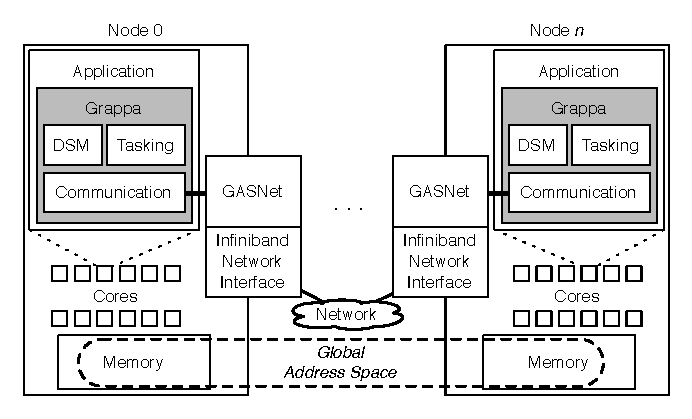
\includegraphics[width=0.95\columnwidth]{figs/system-overview}
\begin{minipage}{0.95\columnwidth}
  \caption{\label{fig:grappa} Grappa system overview}
\end{minipage}
\vspace{-3ex}
\end{center}
\end{figure}


Grappa (Figure~\ref{fig:grappa}) has three main software components:
\begin{description}

\item [Tasking system.] Our tasking system supports lightweight
multithreading to tolerate communication latency and global distributed
workstealing (i.e., tasks can be stolen from any node in the system), which
provides automated load balancing.

\item[Distributed shared memory.] Our DSM system provides support for
fine-grain access to data anywhere in the system. It supports synchronization
operations on global data, explicit local caching of any local in the system,
and support for operation on remote data (delegating operations to home node).
By tight integration with the tasking system described about and the
communication layer (below), our DSM system offers high aggregate random
access bandwidth for accessing remote data.

\item[Communication layer.] As discussed earlier, modern commodity networks
support high bandwidth only for large messages. Since irregular applications
tend to need frequent communication of small requests, the main goal of our
communication layer is to aggregate small messages into large ones better
exploit what the network can offer. It is largely invisible to the application
programmer.

% software developer but helps to improve network performance when applications read and write only small pieces of data.

\end{description}

In the next three sections we describe both the programmer's view of Grappa's main capabilities and how they are implemented.


